\section[绪论]{绪论}
\subsection{h11}
I like u\ucite{Authors2011}
\lipsum[1-10]
自动化\index{auto}
\subsection{h12}

\clearpage
\section{通用样式}
\subsection{字体}
    \subsubsection{字号}
    \subsubsection{字体形状}
    \subsubsection{字体系列}
\subsection{文字修饰}
    \subsubsection{下划线}
    \subsubsection{波浪线}
    % \subsubsection{}
\subsection{列表}
    \subsubsection{有序列表}
    \subsubsection{无序列表}
    % \subsubsection{}
% \subsection{}
\subsection{引用}
\subsection{索引}
% \subsection{}
\clearpage
\section[数学样式]{数学样式}
\subsection{公式}
    \begin{itemize}
        \item 行间公式示例:$E=mc^2$,行间公式不编号
        \item 行内公式示例:\begin{equation}
            E=mc^2
        \end{equation}
        \item 对齐公式:\begin{align}
            y &=(a-b)^2\\
            &=a^2+b^2-2ab \notag\\
            &=(a+b)^2-4ab
        \end{align}
        可以控制是否编号\\notag
    \end{itemize}
   
\subsection{定理}
    \begin{theorem}
        我是一条定理!
    \end{theorem}
    \begin{theorem}
        我是一条定理!
    \end{theorem}
\subsection{引理}
    \begin{lemma}
        我是一条引理!
    \end{lemma}
    \begin{lemma}
        我是一条引理!
    \end{lemma}
\subsection{证明}
    \begin{proof}
        我是一条证明!
    \end{proof}
    \begin{proof}
        我是一条证明!
    \end{proof}
\subsection{命题}
    \begin{props}
        我是命题
    \end{props}
\subsection{猜想}
    \begin{conj}
        我是猜想
    \end{conj}
\subsection{推论}
    \begin{infer}
        我是推论
    \end{infer}
\subsection{定义}
    \begin{defi}
        我是定义
    \end{defi}
\subsection{例}
    \begin{exmp}
        我是例子
    \end{exmp}
\subsection{评论}
    \begin{remark}
        我是评论
    \end{remark}
\subsection{注}
    \begin{note}
        我是注释
    \end{note}
\subsection{断言}
    \begin{asset}
        我是断言
    \end{asset}
\clearpage
\section[代码样式]{代码样式}
\subsection{Python}
\subsection{C++}

\clearpage
\section[图表样式]{图表样式}
\subsection{图}
\lipsum[1]
\begin{figure}[htbp]
    \centering
    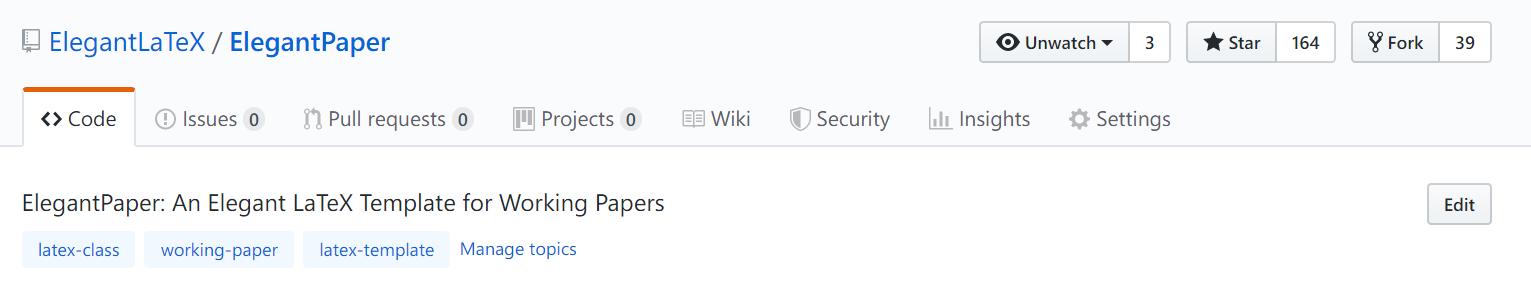
\includegraphics[width=\textwidth]{image/star.png}
    \caption{一键三连求赞}
\end{figure}
\begin{figure}[htbp]
    \centering
    
\includegraphics[scale=.3]{image/donate.jpg}
    \caption{捐赠}
\end{figure}
\lipsum[2]
\subsection{表}
\lipsum[3]
\begin{table}[!htbp]
    \centering
    \caption{Elegant\LaTeX{} 系列模板捐赠榜}
    \begin{tabular}{crcc}
      \toprule
      捐赠者   & 金额 & 时间 & 渠道 \\
      \midrule
      Lerh  & 10 元  & 2019/05/15 & 微信 \\
      越过地平线 & 10 元    & 2019/05/15 & 微信 \\
      大熊 &  20 元 & 2019/05/27 & 微信 \\
      * 空 & 10 元 & 2019/05/30 & 微信\\
      \href{http://www.latexstudio.net/}{latexstudio.net} & 666 元 & 2019/06/05 & 支付宝\\
      Cassis & 11 元 & 2019/06/30 & 微信\\
      * 君 & 10 元 & 2019/07/23 & 微信\\
      * 萌 & 19 元 & 2019/08/28 & 微信 \\
      曲豆豆 & 10 元 & 2019/08/28 & 微信 \\
      李博 & 100 元 & 2019/10/06 & 微信\\
      Njustsll & 10 元 & 2019/10/11 & 微信 \\
    \bottomrule
    \end{tabular}%
  \end{table}%
  \lipsum[4]
% \subsection{}
\clearpage
\section{结论}
